\subsubsection{Por un valor}

Multiplicar una matriz $A$ por un valor $x$ significa que cada elemento de $A$ es multplicado por $x$. Por ejemplo:

$$
2 \cdot \begin{bmatrix}
	6	& 1 & 4 \\
	3 & 9 & 2
\end{bmatrix}   
 = \begin{bmatrix}
 	2 \cdot 6 & 2 \cdot 1 & 2 \cdot 4 \\
 	2 \cdot 3 & 2 \cdot 9 & 2 \cdot 2
 \end{bmatrix} =
\begin{bmatrix}
	6 & 1 & 4 \\
	3 & 9 & 2
\end{bmatrix}$$

\subsubsection{Por otra matriz}

El producto $AB$ de las matrices $A$ y $B$ esta definido si $A$ tiene las dimensiones $a\times n$ y las dimensiones de $B$ es $n \times b$, es decir la cantidad de columnas de $A$ debe ser igual a la cantidad de filas de $B$ para poder efectuar la operación. La operación da como resultado una matriz $C$ de dimensiones $a \times b$ donde cada elemento es calculado usando la siguiente fórmula:

$$ AB[i,j] = \sum_{k=1}^{n}A[i,k]\cdot B[k,j] $$




La idea es que cada elemento de AB es la suma de productos de los elementos de A y B acorde a la siguiente figura:

% TODO: \usepackage{graphicx} required
\begin{figure}[h!]
	\centering
	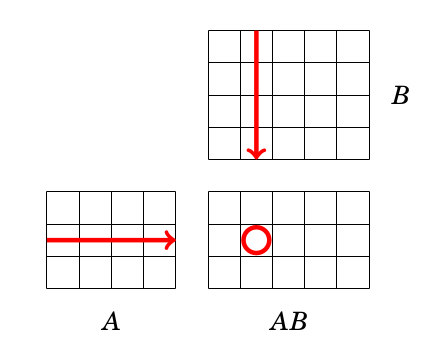
\includegraphics[width=0.5\linewidth]{img/mulmatriz}
	\label{fig:mulmatriz}
\end{figure}

Por ejemplo:
$$
\begin{bmatrix}
   1 & 4 \\
   3 & 9 \\
   8 & 6 
\end{bmatrix}
\cdot
\begin{bmatrix}
	1 & 6 \\
	2 & 9
\end{bmatrix}   
= \begin{bmatrix}
	1 \cdot 1 + 4 \cdot 2  & 1 \cdot 6 + 4 \cdot 9  \\
	3 \cdot 1 + 9 \cdot 2 &  3 \cdot 6 + 9 \cdot 9 \\
	8 \cdot 1 + 6 \cdot 2 &  8 \cdot 6 + 6 \cdot 9 
\end{bmatrix} =
\begin{bmatrix}
	9 & 42 \\
	21 & 99 \\
	20 & 102 
\end{bmatrix}$$

La multplicacion de matrices es asociativa, entonces $A(BC) = (AB)C$ es lo mismo, pero no es conmutativa es decir $AB = BA$ usualmente no es lo mismo. 
